\clearpage
\myparagraph{\olly}
\index{\olly}

\RU{Загрузим этот пример в}\EN{Let's load this example into} \olly. 
\RU{Входное значения для ф-ции пусть будет}\EN{Let the input value be} \TT{0x12345678}.\\
\\
\RU{Для}\EN{For} $i=1$, \RU{мы видим, как}\EN{we see how} $i$ \RU{загружается в}\EN{is loaded into} \ECX: 

\begin{figure}[H]
\centering
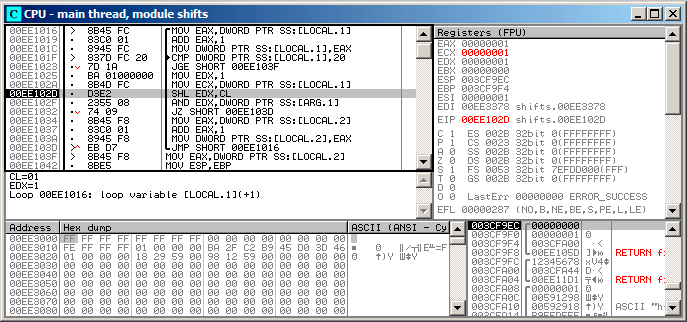
\includegraphics[scale=\FigScale]{patterns/14_bitfields/4_popcnt/olly1_1.png}
\caption{\olly: $i=1$, $i$ \RU{загружено в}\EN{is loaded into} \ECX}
\label{fig:shifts_olly1_1}
\end{figure}

\EDX \RU{содержит}\EN{is} $1$. \RU{Сейчас будет исполнена }\TT{SHL}\EN{ is to be executed now}.

\clearpage
\TT{SHL} \RU{исполнилась}\EN{was executed}:

\begin{figure}[H]
\centering
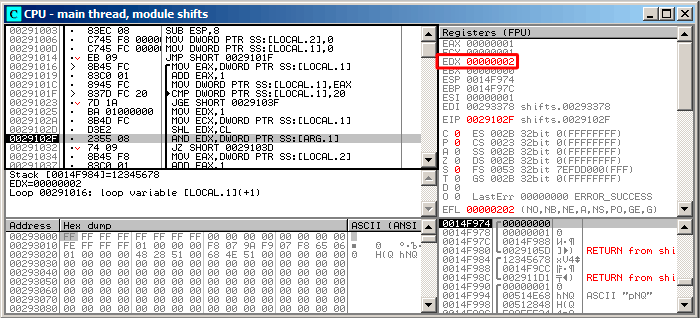
\includegraphics[scale=\FigScale]{patterns/14_bitfields/4_popcnt/olly1_2.png}
\caption{\olly: $i=1$, \EDX=$1 \ll 1=2$}
\label{fig:shifts_olly1_2}
\end{figure}

\EDX \RU{содержит}\EN{contain} $1 \ll 1$ (\OrENRU $2$). \RU{Это битовая маска}\EN{This is a bit mask}.

\clearpage
\ANDIns \RU{устанавливает}\EN{sets} \ZF \RU{в}\EN{to} $1$, 
\RU{что означает, что входное значение}\EN{which means that the input value} (\TT{0x12345678}) 
\RU{умножается\footnote{Логическое ``И''} с}\EN{ ANDed with} $2$ \RU{давая в результате}\EN{results in} $0$:

\begin{figure}[H]
\centering
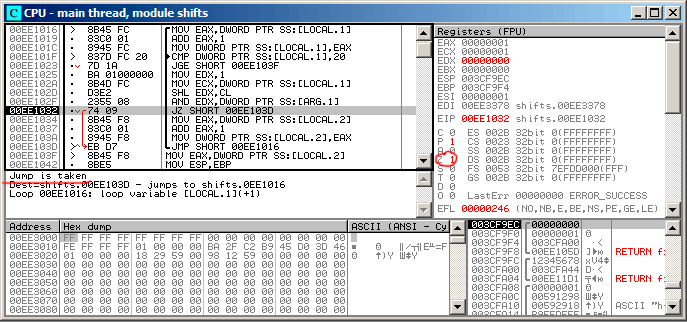
\includegraphics[scale=\FigScale]{patterns/14_bitfields/4_popcnt/olly1_3.png}
\caption{\olly: $i=1$, \RU{есть ли этот бит во входном значении? Нет.}
\EN{is there that bit in the input value? No.} (\ZF=1)}
\label{fig:shifts_olly1_3}
\end{figure}

\RU{Так что, во входном значении соответствующего бита нет}\EN{So, there is no corresponding bit in the input value}.
\RU{Участок кода, увеличивающий счетчик бит на единицу не будет исполнен: инструкция \JZ \textit{обойдет} его}
\EN{The piece of code, which \glslink{increment}{increments} the counter will not be executed: 
the \JZ instruction will \textit{bypass} it}.

\clearpage
\RU{Я немного потрассировал далее и}\EN{I traced a bit further and} $i$ \RU{теперь}\EN{is now} $4$.
\TT{SHL} \RU{исполнилась}\EN{is to be executed now}:

\begin{figure}[H]
\centering
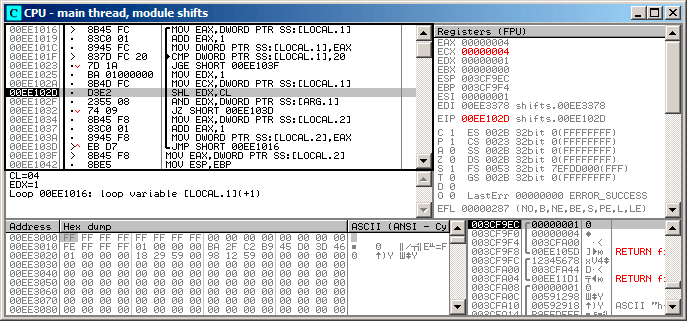
\includegraphics[scale=\FigScale]{patterns/14_bitfields/4_popcnt/olly4_1.png}
\caption{\olly: $i=4$, $i$ \RU{загружено в}\EN{is loaded into} \ECX}
\label{fig:shifts_olly4_1}
\end{figure}

\clearpage
\EDX=$1 \ll 4$ (\OrENRU \TT{0x10} \OrENRU $16$): 

\begin{figure}[H]
\centering
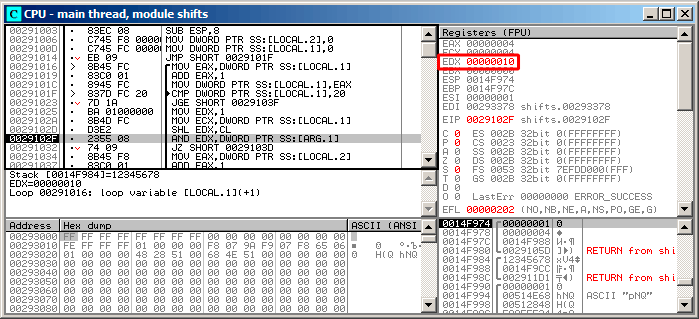
\includegraphics[scale=\FigScale]{patterns/14_bitfields/4_popcnt/olly4_2.png}
\caption{\olly: $i=4$, \EDX=$1 \ll 4=0x10$}
\label{fig:shifts_olly4_2}
\end{figure}

\RU{Это еще одна битовая маска}\EN{This is another bit mask}.

\clearpage
\ANDIns \RU{исполнилась}\EN{is executed}:

\begin{figure}[H]
\centering
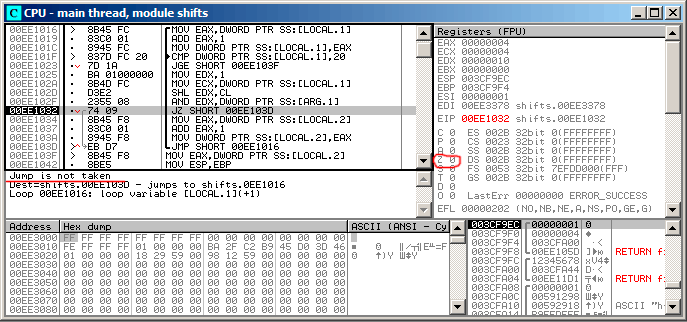
\includegraphics[scale=\FigScale]{patterns/14_bitfields/4_popcnt/olly4_3.png}
\caption{\olly: $i=4$, \RU{есть ли этот бит во входном значении? Да.}
\EN{is there that bit in the input value? Yes.} (\ZF=0)}
\label{fig:shifts_olly4_3}
\end{figure}

\ZF \RU{сейчас}\EN{is} $0$ \RU{потому что этот бит присутствует во входном значении}
\EN{because this bit is present in the input value}.
\RU{Действительно}\EN{Indeed}, \TT{0x12345678 \& 0x10 = 0x10}. 
\RU{Этот бит считается: переход не сработает и счетчик бит будет увеличен на единицу}\EN{This bit counts: 
the jump will not trigger and the bit counter will be \glslink{increment}{incremented} now}.\\
\\
\RU{Ф-ция возвращает}\EN{The function returns} $13$. 
\RU{Это количество установленных бит в значении}\EN{This is total number of bits set in} \TT{0x12345678}.
